\documentclass[12pt,a4paper,draft]{article}

\usepackage[utf8]{inputenc}
\usepackage{mathbbol}
\usepackage[colorlinks=true,linkcolor=blue,citecolor=red,filecolor=magenta,urlcolor=red]{hyperref}
\usepackage{graphicx}
\usepackage{inconsolata}
\usepackage{tcolorbox}
\usepackage{booktabs}
\renewcommand*\contentsname{Indice}

\title{Jollar\footnote{Jollar è un gioco di parole che viene da Jolie + Dollar.} \\ una criptovaluta in Jolie}
\author{Stefano Pio Zingaro}

\begin{document}

\maketitle

\begin{abstract}
\noindent Il progetto di quest'anno propone la creazione un sistema di scambio elettronico decentralizzato, dove gli utenti effettuano transazioni certificate all'interno della rete stessa, senza il bisogno di un organo centrale garante\footnote{Il ruolo che ricoprono le banche nei moderni sistemi finanziari.}. L'implementazione del progetto segue i principi della programmazione orientata ai servizi, rispettandone l'architettura e i paradigmi di gestione della concorrenza. La comunicazione tra i servizi, infine, è implementata nel linguaggio visto a lezione di laboratorio: \href{http://jolie-lang.org}{Jolie}.
\end{abstract}

\tableofcontents

\newpage

\section{Informazioni Logistiche}
\subsection{Formazione dei Gruppi}
%
I gruppi possono essere costituiti da un minimo di 3 a un massimo di 5 persone. 
I gruppi che intendono svolgere questo progetto, devono comunicare via email a \url{stefanopio.zingaro@unibo.it} entro il \textbf{10 Maggio 2018} la composizione del gruppo. 
L'email deve avere come oggetto \textbf{GRUPPO LSO} e contenere:
\begin{enumerate}
    \item Nome del gruppo;
    \item Una riga per ogni componente del gruppo, con cognome, nome e matricola;
    \item Un indirizzo email di riferimento a cui mandare le notifiche al gruppo, sarà poi suo incarico trasmetterle agli altri membri.
\end{enumerate}
Email di esempio con oggetto \textbf{GRUPPO LSO}

\noindent\textit{NomeGruppo}
\begin{itemize}
    \item \textit{Zingaro, Stefano, 123456}
    \item \textit{Pallino, Pinco, 234567}
    \item \textit{Banana, Joe, 345678}
\end{itemize}
\textit{Referente:} \url{stefano.zingaro@studio.unibo.it}

Chi non comunicherà la composizione del gruppo entro il \textbf{10 Maggio 2018} non potrà consegnare il progetto. 
Nel caso, chi non riuscisse a trovare un gruppo, lo comunichi il prima possibile, entro e non oltre il \textbf{7 Maggio 2018}, a \url{stefano.zingaro@studio.unibo.it} con una mail con oggetto \textbf{CERCO GRUPPO LSO}, specificando:
\begin{enumerate}
    \item Cognome, Nome, Matricola, Email;
    \item Eventuali preferenze legate a luogo e tempi di lavoro (si cercherà di costituire gruppi di persone con luoghi e tempi di lavoro compatibili)
\end{enumerate}
Email di esempio con oggetto \textbf{CERCO GRUPPO LSO} 
\begin{itemize}
    \item \textit{Zingaro, Stefano, 123456,} \url{stefano.zingaro@studio.unibo.it}
\end{itemize}
\textit{Preferisco trovarci nei pressi del dipartimento, tutti i giorno dopo pranzo.}

Le persone senza un gruppo verranno raggruppate il prima possibile \textbf{e non sarà possibile modificare i gruppi formati}.
%
\subsection{Date dell'Orale}
%

\newpage

\section{Componenti del Progetto e loro Implementazione}
In generale, il sistema consiste in una rete \textit{Peer-To-Peer} (\textbf{P2P}) che utilizza \textit{Proof-of-Work} (\textbf{POW}) per registrare l'elenco delle transazioni in un archivio pubblico, detto \textbf{blockchain}. Per una migliore comprensione del fenomeno si rimanda alla lettura dell'articolo originale di Satoshi Nakamoto \href{https://bitcoin.org/bitcoin.pdf}{Bitcoin}. 
L'implementazione del progetto è, almeno in parte, ripresa da quella descritta nell'articolo, fatta eccezione per lo sviluppodella Proof-of-Work, che segue i principi della criptovaluta \href{http://primecoin.io/bin/primecoin-paper.pdf}{\textbf{Primecoin}}.

In questa sezione sono enunciate le definizioni di transazioni (contenute in un blocco) e blockchain, e se ne discute la relativa implementazione. Sono poi elencate le definizioni delle altre componenti del sistema: il meccanismo di convalida di un blocco (la Proof-of-Work); il server Timestamp per la sincronizzazione oraria; il comportamento della rete all'avvio dell'esecuzione.

\subsection{Le transazioni e la catena di blocchi: la Blockchain}
La \textbf{blockchain} è una struttura dati ordinata, una lista concatenata di blocchi contenenti transazioni. L'intera struttura della blockchain può essere conservata in un file, oppure in un database. Un \textbf{block}, o blocco, è un contenitore, una struttura dati a sua volta, che aggrega transazioni che devono essere incluse in un \textit{ledger}\footnote{Il termine ledger indica il libro mastro dei contabili, viene tradotto in italiano come registro.} pubblico e condiviso, la blockchain. 
Il blocco è composto da un \textit{header}, che contiene i \textit{metadata}, e dalla lista di transazioni che ne compongono la maggior parte della grandezza. Di seguito un esempio in Jolie di un tipo ``custom''.

\subsubsection{Implementazione}
\begin{enumerate}
    \item L'ID del blocco;
    \item Il hash del blocco precedente;
    \item Lunghezza della Proof-of-Work;
    \item Il numero primo origine (descritto più avanti);
    \item La catena di numeri primi che compone la Proof-of-Work di quel blocco;
\end{enumerate}

%
\lstinputlisting[language=Jolie]{code/block.ol}
%

\noindent In Jolie la funzione di Hash MD5 (da 128 bit) si trova già implementata nell'interfaccia \texttt{MessageDigest}.
%
\lstinputlisting[language=Jolie]{code/hash.ol}
%

\subsection{Il Server Timestamp}
Un server timestamp offre un servizio che permette di conoscere l'ora esatta all'interno della rete. Un nodo che intende effettuare le operazioni di scrittura o di validazione di un blocco deve richiedere il \textbf{timestamp} al server. Esso garantisce l'esistenza dei dati al momento della richiesta.

\subsubsection{Implementazione}
In particolare, Jolie offre, tramite l'interfaccia \texttt{time} una \texttt{operation} che restituisce i millisecondi del \textit{current unix timestamp} nel momento esatto della richiesta. Tramite una chiamata a tale servizio si può ottenere il dato necessario da includere nel blocco. Qui è riportato un esempio si chiamata a tale operation, che può essere inserita in un server che accetta richieste e le inoltra al servizio time.
%
\lstinputlisting[language=Jolie]{code/timestamp.ol}
%

\subsection{La Proof-of-Work}
La Proof-of-Work, è un algoritmo che viene utilizzato per raggiungere un accordo decentralizzato tra diversi nodi nel processo di aggiunta di un blocco specifico alla blockchain.
Tale algoritmo produce valori che vengono utilizzati per verificare che sia stata eseguita una notevole quantità di lavoro. Nell'immagine riportata qui sotto viene visualizzato un esempio di utilizzo di tecniche Proof-of-Work nel mondo delle criptovalute (in particolare quella di Ethereum ma generalizzabile a qualunque altra che usa Proof-of-Work).
Per implementare un sistema decentralizzato basato su rete P2P, abbiamo bisogno di usare un sistema di Proof-of-Work\footnote{\url{http://www.wisdom.weizmann.ac.il/~naor/PAPERS/pvp.ps}}. Questo metodo consiste nell'obbligare i nodi che vogliono scrivere un blocco a cercare un valore che sia difficile da trovare e di cui sia facile controllarne la correttezza da parte degli altri nodi che vogliono validare la scrittura.
\begin{center}
    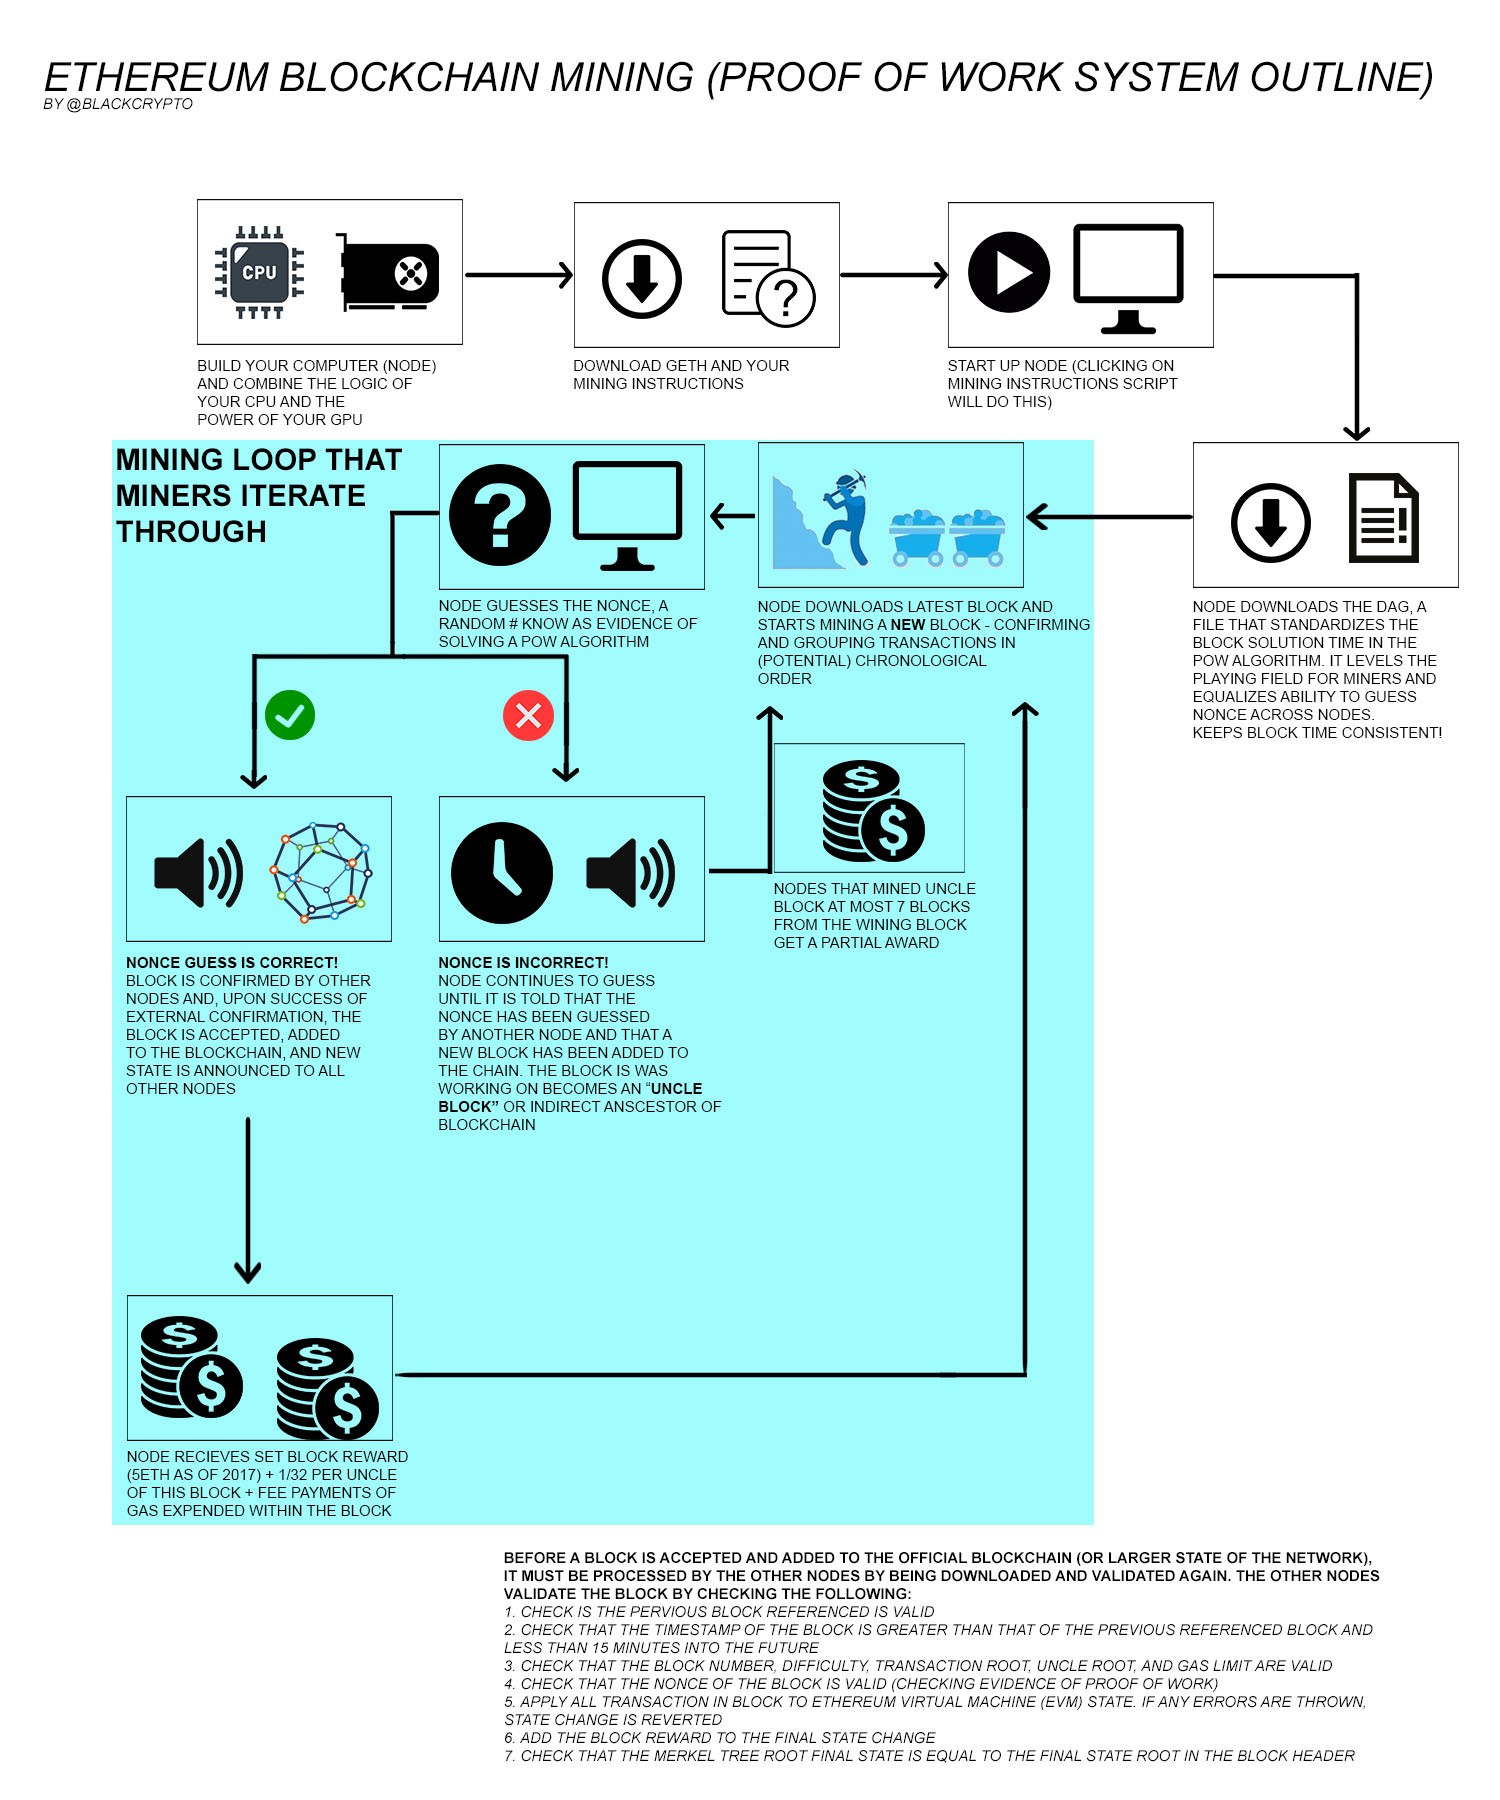
\includegraphics[width=\linewidth]{img/pow}
\end{center}

\subsubsection{Implementazione}
La Proof-of-Work scelta per produrre blocchi ed ottenere così sei Jollar in \textit{reward}\footnote{A differenza di Bitcoin, il reward in questo caso è fissato a sei ed è costante per tutta la vita della rete, un \textit{improvement} possibile è cambiare questo valore in una funzione decrescente.} è quella utilizzata dalla moneta PrimeCoin. Essa consiste nel generare delle catena di numeri primi con determinate proprietà.

\subsubsection*{Catene di Cunningham del Primo Tipo}
Una catena di Cunningham del primo tipo di lunghezza $k$ è un array di numeri primi:
\begin{center}
    $n-1,2n-1,\dots,2^{k-1}n-1$
\end{center}
Il numero $n$ è chiamato l'\textbf{origine} della catena. L'origine di una catena va va incluso nel blocco! Un esempio:
\begin{itemize}
    \item origine: $n=5$
    \item lunghezza: $k=5$
    \item catena: $2,5,11,23,47$
\end{itemize}

\subsubsection*{Catene di Cunningham del Secondo Tipo}
Una catena di Cunningham del secondo tipo di lunghezza $k$ è un array di numeri primi:
\begin{center}
    $n-1,n+1,2n-1,2m+1,\dots,\dots,2^{k-1}n-1,2^{k-1}n+1$
\end{center}
Un esempio:
\begin{itemize}
    \item origine: $n=4$
    \item lunghezza: $2k=4(k=2)$
    \item catena: $5,7,11,13$
\end{itemize}

\subsubsection*{Catene Bi-twin}
Una catena di Bi-twin di lunghezza $2k$ è una catena di $k$ numeri primi
\begin{center}
    $n-1,2n-1,\dots,2^{k-1}n-1$
\end{center}
 Un esempio:
\begin{itemize}
    \item origine: $n=5$
    \item lunghezza: $k=5$
    \item catena: $5,7,11,13$
\end{itemize}
Le catene Bi-twin posso anche essere viste come l'unione di due catene di Cunningham del primo o del secondo tipo con la stessa origine e lunghezza.
%
\subsection*{Validazione delle catene}
Il meccanismo di controllo e validazione delle Proof-of-Work inviate contenenti le catene di numeri primi prevede un test che utilizza il piccolo Teorema di Fermat (\href{http://primes.utm.edu/notes/proofs/FermatsLittleTheorem.html}{link alla dimostrazione}), esso afferma che, per $p$ primo ed $a$ intero 
\begin{center}
$a^{p-1} \equiv 1 (\bmod p)$ se $p$ non divide $a$.
\end{center}

\noindent I $p$ che soddisfano questo proprietà vengono chiamati \textit{pseudoprimi}, perché non tutti sono appunto primi. Vale però che maggiore è $p$, maggiore è la probabilità che sia primo. 

\noindent Un esempio utilizza tipicamente $a=2$ e lo eleva alla $p-1$ (prendiamo $17$ e $23$) che modulo p risulta essere uguale ad $1$:
\begin{center}
$2^{16}= 65536 \bmod 17 = 1$ \\
oppure \\
$2^{22}= 4194304 \bmod 23 = 1$
\end{center}

Ciò significa che per la primalità va controllata per ogni numero primo della catena. Inoltre la validazione controlla anche che la lunghezza della catena sia maggiore o uguale alla difficoltà (quindi il tipo di catena va incluso nel blocco!)

\subsection{La Rete Peer-To-Peer}
Una rete P2P, come ad esempio quella di \href{www.emule-project.net/home/perl/}{Emule}, è una rete i cui nodi non sono \textbf{client} o \textbf{server} fissi, ma prendono forma di entità equivalenti o ``paritarie''.
\begin{center}
    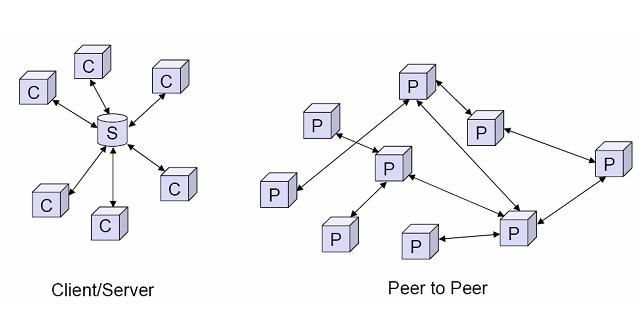
\includegraphics[width=\linewidth]{img/p2p}
\end{center}

\subsubsection{Implementazione}
L'esecuzione della rete P2P comprende i seguenti passaggi:
\begin{enumerate}
    \item Le nuove transazioni sono inviate in \textit{broadcast}\footnote{Nelle reti di calcolatori, il termine broadcast indica una modalità di instradamento per la quale un pacchetto dati inviato ad un indirizzo particolare (detto appunto di broadcast) verrà consegnato a tutti i computer collegati alla rete} a tutti i nodi che partecipano alla rete;
    \item Ogni nodo colleziona la nuove transazione in un blocco (una transazione per blocco!);
    \item Ogni nodo effettua del ``lavoro'' per provare di poter scrivere il blocco (Proof-of-Work);
    \item Quando un nodo trova una prova, invia il blocco in broadcast a tutti i nodi;
    \item I nodi accettano il nuovo blocco solo se la transazione contenuta in esso è valida e non è stata già ``spesa'';
\end{enumerate}

I nodi considerano sempre la blockchain più lunga come quella corretta. Nel caso in cui due nodi inviano versioni differenti del nuovo blocco contemporaneamente, alcuni nodi potrebbero riceverne  una versione, altri l'altra. In quel caso il nodo lavora sul blocco ricevuto temporalmente prima. Il nodo che ha lavorato su un blocco non sincronizzato se ne rende conto quando una nuova validazione viene richiesta, in questo caso egli manda in broadcast una richiesta di sincronizzazione sul blocco in questione e, una volta ricevuta risposta, aggiorna la blockchain alla versione più recente, potendo così validare il nuovo blocco ricevuto.

\subsection{Il Network Visualiser}
Il Network Visualiser è un tool amministrativo da terminale per il monitoraggio del sistema.

\subsubsection{Implementazione}
Il Network Visualizer invia richieste a tutta la rete per conoscere lo stato delle blockchain di tutti i nodi, la loro versione, le transazioni che contengono, generando le seguenti informazioni:
\begin{itemize}
    \item La data e l'ora del server timestamp al momento della richiesta.
    \item Per ogni utente/nodo: la sua chiave pubblica; le transazioni che ha effettuato divise per entrate/uscite; la versione della blockchain che utilizza e la quantità totale di Jollar che possiede.
    \item Per ogni transazione al punto precedente, ordinate in ordine cronologico, si indica la data, l'ora, e gli utenti (con le loro chiavi pubbliche) coinvolti.
    \item La blockchain più lunga presente nella rete (chiamata la versione ufficiale), con tutta la struttura dati che contiene.
\end{itemize}

\newpage

\section{Specifiche di Consegna}
Globalmente vengono consegnati tre prodotti: il report del progetto, la sua implementazione in codice Jolie ed una demo di funzionamento. La valutazione finale avviene mediante una discussione di gruppo.
\begin{tcolorbox}[colback=yellow!20!white,colframe=yellow!75!black,title=\textbf{N.B.}]
    \begin{enumerate}
        \item non si accettano richieste di eccezioni sui progetti con motivazioni legate a esigenze di laurearsi o di non voler pagare le tasse per un altro anno.
        \item chi copia o fa copiare, anche solo in parte, si vede invalidare completamente il progetto senza possibilità di appello $\rightarrow$ deve quindi rifare un nuovo progetto l'anno successivo.
    \end{enumerate}
\end{tcolorbox}

\subsection{Il Report}
È possibile scrivere il report nel formato preferito, l'importante è che il PDF generato rispetti la struttura del modello (riportato qui in basso). Il report ha lunghezza di quattro o cinque pagine (quindi da 8 a 10 facciate), è scritto con font di grandezza \textbf{12pt} e viene consegnato in formato PDF. 
Di seguito viene riportato un esempio di report con le principali caratteristiche da inserire.
\begin{tcolorbox}[colback=green!20!white,colframe=green!75!black,title=L'intestazione del Report]
\begin{itemize}
    \item Jollar -- Laboratorio Sistemi Operativi A.A. 2017-2018
    \item Nome del Gruppo
    \item Indirizzo mail di riferimento: myaccount@email.com
    \item Componenti:
    \begin{itemize}
        \item Cognome, Nome, Matr. 0000424242
        \item \dots
    \end{itemize}
\end{itemize}
\end{tcolorbox}
\begin{tcolorbox}[colback=green!20!white,colframe=green!75!black,title=Il corpo del Report]
\begin{enumerate}
    \item Descrizione generale del progetto -- descrizione delle features implementate e del contenuto del report.
    \item Istruzioni per la demo -- le istruzioni per eseguire una demo.
    \item Discussione sulle strategie di implementazione 
    \begin{enumerate}
        \item Struttura del progetto -- come è stato diviso il progetto, perché, i problemi principali riscontrati, le alternative considerate e le soluzioni scelte.
        \item Sezione di descrizione della feature x -- abbiamo implementato la funzione di `foo` \dots (con esempi di codice).
    \end{enumerate}
\end{enumerate}
\end{tcolorbox}

\subsubsection{Griglia di Valutazione}
La valutazione del report verte sull'analisi dello scritto e sulla sua capacità di esprimere con chiarezza i concetti descritti, soprattutto grazie all'uso di esempi. In particolare la griglia di valutazione usata è la seguente:
\newpage
\begin{table}[ht]
    \centering
    {\footnotesize
    \begin{tabular}{|l|l|l|l|}
    \hline
    \multicolumn{1}{|c|}{\textbf{Indicatore}}                                                  & \multicolumn{1}{c|}{\textbf{Livello 1}}                                                                                                                                  & \multicolumn{1}{c|}{\textbf{Livello 2}}                                                                                                                    & \multicolumn{1}{c|}{\textbf{Livello 3}}                                                                                                                    \\ \hline
    \textit{\begin{tabular}[c]{@{}l@{}}Qualità \\ dell'informazione\end{tabular}}              & \begin{tabular}[c]{@{}l@{}}Mancato\\ riconoscimento\\ dei problemi \\ (di concorrenza)\\ e assenza della\\ loro descrizione.\end{tabular}                                & \begin{tabular}[c]{@{}l@{}}Riconoscimento\\ dei problemi \\ (di concorrenza)\\ e assenza della\\ loro descrizione.\end{tabular}                            & \begin{tabular}[c]{@{}l@{}}Riconoscimento\\ dei problemi\\ (di concorrenza)\\ e presenza della\\ loro descrizione.\end{tabular}                            \\ \hline
    \textit{\begin{tabular}[c]{@{}l@{}}Uso degli \\ esempi\end{tabular}}                       & \begin{tabular}[c]{@{}l@{}}Assenza di\\ esempi a\\ supporto delle\\ scelte\\ implementative.\end{tabular}                                                                & \begin{tabular}[c]{@{}l@{}}Presenza di\\ esempi in\\ alcune ma non\\ tutte le\\ scelte\\ implementative.\end{tabular}                                      & \begin{tabular}[c]{@{}l@{}}Presenza di\\ almeno un \\ esempio in\\ tutte le scelte\\ implementative.\end{tabular}                                          \\ \hline
    \textit{\begin{tabular}[c]{@{}l@{}}Analisi \\ delle scelte \\ implementative\end{tabular}} & \begin{tabular}[c]{@{}l@{}}Assenza della \\ descrizione della \\ propria scelta \\ implementativa \\ ed assenza \\ di proposte \\ di alternative \\ valide.\end{tabular} & \begin{tabular}[c]{@{}l@{}}Descrizione \\ della propria \\ scelta \\ implementativa \\ ed assenza \\ di proposte \\ di alternative \\ valide.\end{tabular} & \begin{tabular}[c]{@{}l@{}}Descrizione \\ della propria \\ scelta \\ implementativa \\ e presenza \\ di proposte \\ di alternative \\ valide.\end{tabular} \\ \hline
    \end{tabular}
    }
\end{table}

\subsection{L'Implementazione}
Il progetto viene sviluppato utilizzando il linguaggio Jolie. Non ci sono requisiti riguardo ai protocolli (\textit{protocol}) e i media (\textit{location}) utilizzati per realizzare la comunicazione tra i componenti del sistema. La gestione del progetto avviene col supporto del sistema \textit{git}. Il codice del progetto è contenuto in un repository su \href{http://gitlab.com}{GitLab} e viene gestito seguendo la procedura descritta sotto.
%
\begin{tcolorbox}[colback=blue!20!white,colframe=blue!75!black,title=GitLab]
\begin{itemize}
    \item Ogni membro del gruppo crea un account su GitLab;
    \item il referente del gruppo  crea un nuovo progetto cliccando sul \textbf{+} in alto a destra nella schermata principale di GitLab, inserendo il nome ``LabSO\_NomeGruppo'' e cliccando su \textbf{New Project};
    \item una volta che il progetto è stato creato, il referente aggiunge ogni membro del gruppo come \textbf{role permission} $>$\textbf{Developer} al progetto andando su \textbf{Settings} $>$ \textbf{Members} nel menù a sinistra, cercandoli in base allo username registrato su GitLab;
    \item il referente aggiunge l'utente ``stefanopiozingaro'' come \textbf{role permission} $>$ \textbf{Reporter}.
\end{itemize}
\end{tcolorbox}
%
Al momento della consegna, il repository dovrà contenere i sorgenti del progetto e la relazione, nominata \textbf{REPORT\_LSO.pdf}. Per effettuare la consegna:
\begin{enumerate}
    \item nella pagina di GitLab del repository, cliccare sulle voci del menù \textbf{Repository} $>$ \textbf{Tags} $>$ \textbf{New Tag}; 
    \item digitare come \textbf{Tag Name} il nome \textbf{Consegna};
    \item cliccare su \textbf{Create Tag} per eseguire la creazione del \textbf{Tag} di consegna.
\end{enumerate}
%
Una volta creato il Tag, inviare una email di notifica di consegna con soggetto \textbf{CONSEGNA LSO - NOME GRUPPO} a \href{stefanopio.zingaro@unibo.it}{questo indirizzo di posta elettronica}. 
\begin{tcolorbox}[colback=yellow!20!white,colframe=yellow!75!black,title=\textbf{N.B.}]
    Il report va anche consegnato in forma cartacea nella casella del prof. Sangiorgi al piano terra del Dipartimento di Informatica, a fianco del suo ufficio.
\end{tcolorbox}

\subsubsection{Griglia di Valutazione} 
La valutazione dell'implementazione del sistema si basa sull'analisi del codice Jolie, sull'uso dei costrutti del linguaggio per la creazione di soluzioni efficienti, sulla tolleranza ai guasti del sistema implementato e sulla gestione degli errori. In particolare la griglia di valutazione usata è la seguente:
\newpage
\begin{table}[ht]
    \centering
    {\footnotesize
    \begin{tabular}{|l|l|l|}
\hline
\multicolumn{1}{|c|}{\textbf{Indicatore}}                                                            & \multicolumn{1}{c|}{\textbf{Livello 1}}                                                                                                                                                & \multicolumn{1}{c|}{\textbf{Livello 2}}                                                                                                                              \\ \hline
\textit{\begin{tabular}[c]{@{}l@{}}Uso dei\\ costrutti\\ di Jolie\end{tabular}}                      & \begin{tabular}[c]{@{}l@{}}Mancato utilizzo\\ dei costrutti per la\\ gestione del\\ parallelismo, uso di \\ execution(sequential)\\ in alcuni servizi \\ ma non in tutti.\end{tabular} & \begin{tabular}[c]{@{}l@{}}Corretto utilizzo\\ dei costrutti per la\\ gestione del\\ parallelismo, uso di\\ execution(concurrent)\\ in tutti i servizi.\end{tabular} \\ \hline
\textit{\begin{tabular}[c]{@{}l@{}}Distribuzione\\ del carico\\ di lavoro\\ nel gruppo\end{tabular}} & \begin{tabular}[c]{@{}l@{}}Disomogeneità\\ nella ripartizione del\\ lavoro nel gruppo, \\ con conseguente \\ dissimmetria di\\ informazione.\end{tabular}                              & \begin{tabular}[c]{@{}l@{}}Omogeneità nella\\ ripartizione dei \\ compiti nel gruppo,\\ ogni membro \\ partecipa egualmente\\ allo sviluppo.\end{tabular}            \\ \hline
\textit{\begin{tabular}[c]{@{}l@{}}Grado di \\ partecipazione\\ alla comunità\end{tabular}}          & \begin{tabular}[c]{@{}l@{}}Assenza di domande\\ e risposte sul \\ newsgroup del corso\end{tabular}                                                                                     & \begin{tabular}[c]{@{}l@{}}Presenza di domande \\ e risposte sulla\\ newsgroup del corso\end{tabular}                                                                \\ \hline
\end{tabular}
    }
\end{table}

\subsection{La Demo}
La demo, o dimostrazione di funzionamento, esegue e monitora il comportamento di un sistema di gestione decentralizzata di transazioni. Essa simula almeno quattro utenti che entrano a far parte della rete peer-to-peer come nodi, un server timestamp che gestisce la sincronizzazione oraria ed un tool per monitorare lo stato della rete (il Network Visualiser).
La sequenza di esecuzione è la seguente:
\begin{enumerate}
    \item avvio del Server Timestamp;
    \item avvio del Network Visualizer;
    \item avvio del primo nodo, generatore del primo blocco (con \textit{reward} di sei Jollar);
    \item avvio del secondo, terzo e quarto nodo (con conseguente \textit{download} della blockchain);
    \item invio di un Jollar dal primo al secondo nodo (con conseguente scrittura su un nuovo blocco e reward relativo);
    \item invio di due Jollar dal primo al terzo nodo (con conseguente scrittura su un nuovo blocco e reward relativo);
    \item invio di tre Jollar dal primo al quarto nodo (con conseguente scrittura su un nuovo blocco e reward relativo);
    \item richiesta al Network Visualiser di stampare la situazione relativa al totale dei Jollar presenti nella rete e dei relativi possessori, con l'elenco delle transazioni avvenute.
\end{enumerate}

\end{document}